\section{IDE set up}

\begin{frame}
\frametitle{Follow the TODOs}
\begin{itemize}
 \item Track the TODO in the *-start projects!
 \item It's easier with support from the IDE
\end{itemize}

\begin{figure}
\begin{center}
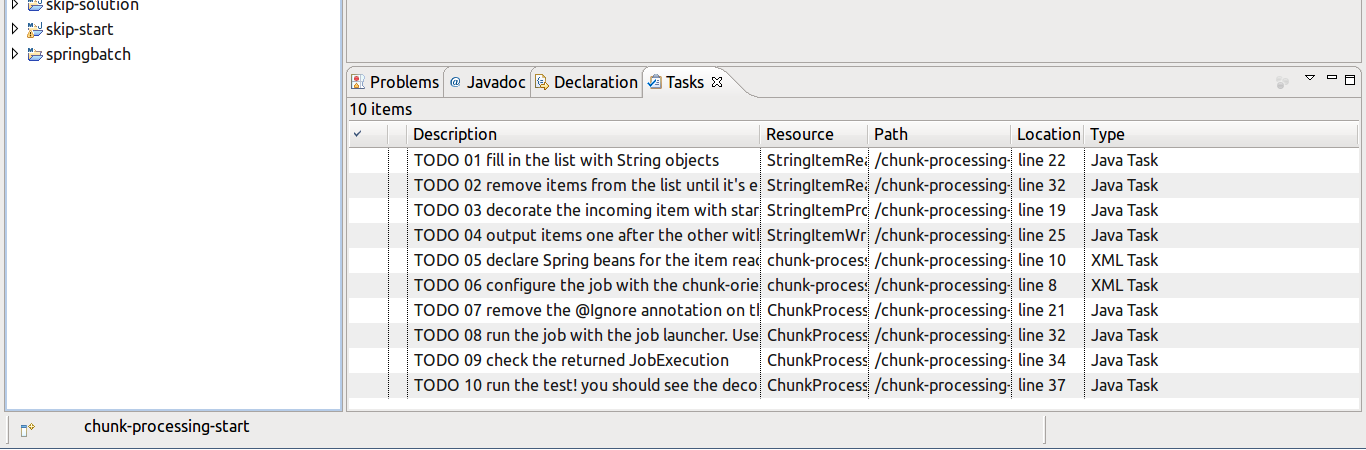
\includegraphics[width=10cm]{figures/tasks.png}
\end{center}
\end{figure}
 
\end{frame}

\begin{frame}
\frametitle{TODO with Eclipse}
\begin{itemize}
 \item Window \textgreater \space Preferences \textgreater \space ``tasks tag'' in filter   
\end{itemize}

\begin{figure}
\begin{center}
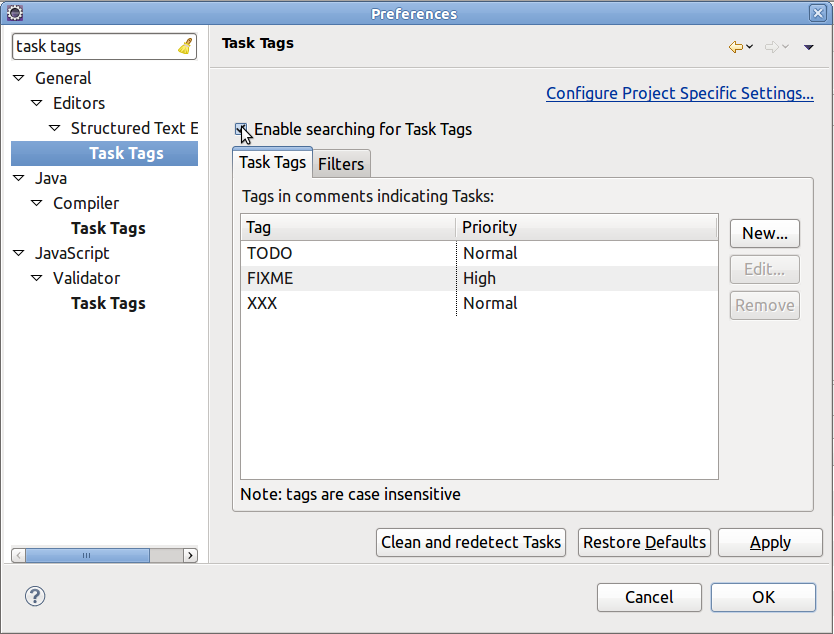
\includegraphics[width=8cm]{figures/enable-task-tags.png}
\end{center}
\end{figure}

\end{frame}
 
\begin{frame}
\frametitle{TODO with Eclipse}
\begin{itemize}
 \item Open the ``Tasks'' view 
 \item click on the down arrow on the right
 \item ``configure contents''
\end{itemize}

\begin{figure}
\begin{center}
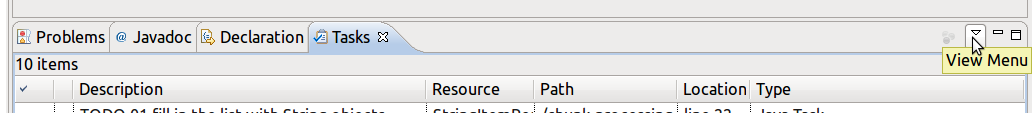
\includegraphics[width=8cm]{figures/configure-content.png}
\end{center}
\end{figure}

\end{frame}

\begin{frame}
\frametitle{TODO with Eclipse}
\begin{itemize}
 \item Check ``TODOs'' on the left
 \item Check ``On any element in the same project'' on the right (scope)
\end{itemize}

\begin{figure}
\begin{center}
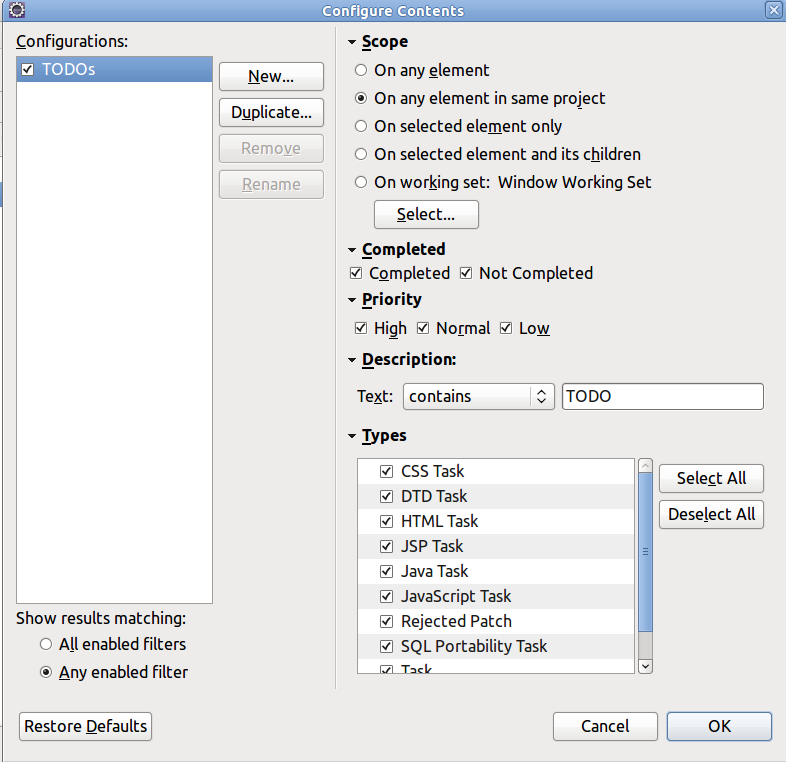
\includegraphics[width=5cm]{figures/content.png}
\end{center}
\end{figure}


\end{frame}